\documentclass[__main__.tex]{subfiles}

\begin{document}

\section{Конечный элемент для одинаковой аппроксимации каждой компоненты вектор-функции. Вид операторов P K -интерполяции и табуляции. Метод конечных элементов для краевой задачи для стационарного уравнения линейной теории упругости с граничными условиями первого и второго рода. Матричная запись вариационного уравнения. Вывод разрешающей СЛАУ. Глобальная и локальная СЛАУ.}

\begin{definition}
    (Оператор интерполяции в КЭ) Пусть ($K$, $P_k$, $\Sigma_k$) -- конечный элемент. Тогда $\forall x \in C^s(K)$ определен оператор:
    \begin{gather*}
        (\Pi_k \cdot x)(\tau) =\sum_{i=1}^N f_i(x)\varphi_i(\tau) \qquad \forall \tau \in K 
    \end{gather*}
    По определению КЭ 
    \begin{gather*}
        \Pi_k \cdot p = p \qquad \forall p \in P_k
    \end{gather*}
\end{definition}

\begin{definition}
    (Оператор табуляции в КЭ) Пусть ($K$, $P_k$, $\Sigma_k$) -- конечный элемент. Тогда оператор 
    \begin{gather*}
        T_k: \ C^s(\Omega) \rightarrow \mathbb{R}^N
    \end{gather*}
    является оператором табуляции, если 
    \begin{gather*}
        T_K(x) = \left(
        \begin{matrix}
            f_1(x)\\
            \vdots \\
            f_n(x)
        \end{matrix}    
        \right)
    \end{gather*}
    Если ($K$, $P_k$, $\Sigma_k$) -- КЭ, то оператор интерполяции записывается в виде:
    \begin{gather*}
        \Pi_k \cdot x = \sum^n_{i=1} f_i(x) \varphi_i = \varphi^T \cdot T_k(x), 
    \end{gather*}
    где 
    \begin{gather*}
        \varphi(\tau) = \left(
            \begin{matrix}
                \varphi_1(\tau)\\
                \vdots \\
                \varphi_n(\tau)
            \end{matrix}    
            \right)
    \end{gather*}
\end{definition}

\subsection{Краевая задача трехмерной линейной упругости в малых деформациях}

Пусть $\Omega \subset \mathbb R^3$, $\partial \Omega = \Sigma_u \cup \Sigma_\sigma$\\
$f \in C(\Omega)$\\
$\overbar t_e \in [C(\Sigma_\sigma)]^3$\\
$\overbar u \in [C(\\Sigma_u)]^3$\\
$^4C=C^{ijkl}\overbar e_i \otimes \overbar e_j \otimes \overbar e_k \otimes \overbar e_l$
Тогда ставится задача определения $\overbar u \in [C^2(\Omega) \cap C(\overbar \Omega)]^3$, что:
\begin{gather*}
    \begin{cases}
        \nabla \cdot \sigma = \overbar f_i, \ \forall \tau \in \Omega \hfill \\
        \tilde{\sigma} =^4\tilde C \cdot \cdot \varepsilon, \forall \tau \in \Omega \hfill \\
        2 \varepsilon = \nabla \otimes \overbar u + (\nabla \otimes \overbar u)^T, \forall \tau \in \Omega \hfill \\
        \tilde{\sigma} \overbar u |_{\Sigma_\sigma} = \overbar t_e, \ \forall \tau \in \Omega \hfill \\
        \overbar u |_{\Sigma_{u}} = \overbar u_e, \ \forall \tau \in \Omega \hfill \\
    \end{cases}
\end{gather*}
Необходимо перейти к вариационной формулировке. Пусть $\vec{v} \in [C^1(\Omega)]^3$ и $\vec v |_{\Sigma_u}=0$. \\
Домножим на $\vec v$ уравнения системы и проинтегрируем:
\begin{gather*}
    \int_{\Omega} (\nabla \cdot \sigma)\vec v d \tau = \int_{\Omega} \vec f \cdot \vec v d \tau  
\end{gather*}
так как $\nabla(\tilde{\sigma}\cdot \vec v) =(\nabla \cdot \tilde{\sigma}\cdot \vec v) + \tilde{\sigma}\cdot \cdot \varepsilon(\vec v)$:
\begin{gather*}
    \int_{\Omega} \nabla (\tilde{\sigma}\cdot \vec v) d \tau - \int_{\Omega} \tilde{\sigma}\cdot \cdot \varepsilon(\vec{v})d\tau = \int_{\Omega} \vec f \cdot \vec v d\tau \\
\end{gather*}
бля мне влом печатать дальше, поэтому вставлю скрин
\begin{figure}[H]
    \begin{centering}
        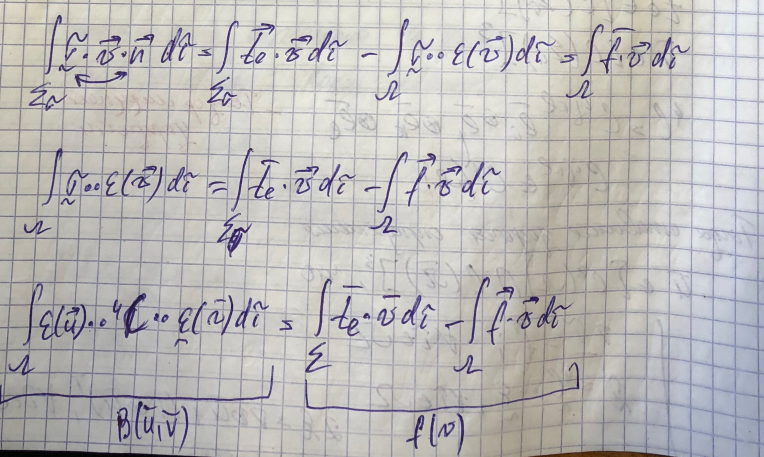
\includegraphics[width=10cm]{16}
    \end{centering}
\end{figure}
\end{document}
